\documentclass{article}
\usepackage[utf8]{inputenc}
\usepackage[czech]{babel}
\usepackage[dvipsnames]{xcolor}

\usepackage{graphicx}
\usepackage{amsthm}
\usepackage{amsmath}
\def\baselinestretch{1}\normalsize 
\usepackage{wrapfig}
\usepackage{pgf,tikz} 
\usepackage{dsfont}

\usepackage[bottom]{footmisc}
\usepackage{footnote}
\usepackage{textcomp}
\usepackage{amssymb}
\usepackage{url}
\usepackage{float}
\usepackage{caption}
\usepackage{subcaption}
\usepackage{multirow}
\usepackage[total={17cm,25cm}, top=3cm, left=2.5cm, right=2.5cm, bottom = 2cm, includefoot]{geometry}
\usepackage{nicefrac}

\usepackage{braket}

\usepackage{centernot}
\usepackage{mathtools}

\newcommand{\incfig}[1]{%
    \def\svgwidth{\columnwidth}
    \import{./figures/}{#1-1.png_tex}
}



\definecolor{Ao}{rgb}{0.0, 0.5, 0.0}

\begin{document}
\begin{center}
    \Large
    \textbf{Poznámky k BEC článkům}
           
    \vspace{0.4cm}
    \small
    \textbf{5. května 2021}
\end{center}

\section{Bose-Einsteinův kondenzát - BEC}
Pro spin $F = I + J$, - spin jádra a obalu. Pro $F = 1$ zavádíme tři sadu kreačních a anihilačních operátorů $\hat{a}_0,\hat{a}_{\pm}$

Hamiltonián kondenzátu 

\begin{aligned}
    \hat{H}=& g\left\{\left(\hat{a}_{0}^{\dagger} \hat{a}_{0}^{\dagger} \hat{a}_{1} \hat{a}_{-1}+\hat{a}_{1}^{\dagger} \hat{a}_{-1}^{\dagger} \hat{a}_{0} \hat{a}_{0}\right)+\hat{N}_{0}\left(\hat{N}_{1}+\hat{N}_{-1}\right)\right.\\
    &\left.+\frac{1}{2}\left(\hat{N}_{1}-\hat{N}_{-1}\right)^{2}\right\}+q\left(\hat{N}_{1}+\hat{N}_{-1}\right) \\
    &+\frac{r}{\sqrt{2}}\left\{\left(\hat{a}_{1}^{\dagger}+\hat{a}_{-1}^{\dagger}\right) \hat{a}_{0}+\hat{a}_{0}^{\dagger}\left(\hat{a}_{1}+\hat{a}_{-1}\right)\right\}
    \end{aligned}

    Ten odpovídá hybnostní reprezentaci vibronového hamiltoniánu s algebrou $(\hat{R}_+,\hat{R}_-,\hat{l})$ v řetězci.

    $$\frac{1}{2}(\hat{R}_+\hat{R}_- + \hat{R}_+\hat{R}_-) + \hat{l}^2 = 
    2(\tau_+^{\dagger} \tau_-^{\dagger} \sigma \sigma + N_+ N_{\sigma} + N_- N_{\sigma}
     +\tau_+ \tau_- \sigma^{\dagger} \sigma^{\dagger} ) + \textcolor{red}{2N -n} + (N_+ - N_-)^2$$

     \begin{aligned}
        \hat{H}_{\text{vibron}}=& \frac{g}{2} \hat{W}^2(\hat{R}_+,\hat{R}_-,\hat{l}) -\frac{g}{2} (\textcolor{red}{2N -n} )
       +q\hat{n} 
        +\frac{r}{\sqrt{2}}(\hat{R}_+ + \hat{R}_-)
        \end{aligned}

        Bez konstanty $N$ tak máme

        \begin{aligned}
            \hat{H}_{\text{vibron}}= (q + \frac{g}{2})\hat{n} + \frac{g}{2} \hat{W}^2(\hat{R}_+,\hat{R}_-,\hat{l})
            +\frac{r}{\sqrt{2}}(\hat{R}_+ + \hat{R}_-)
            \end{aligned}

$q,g,r$ jsou parametry interakce daných bosonových atomů (na experiment Rubidium 87).

\section{Rozdíl mezi $\hat{H}(\hat{D}_{\pm})$ a $\hat{H}(\hat{R}_{\pm})$}
Zajímá nás rozdíl ve vlastnostech operátorů

$$\hat{H}_D = (1 - \xi)\hat{n} - \frac{\xi}{N - 1}\bigg( \frac{1}{2}(\hat{D}_+\hat{D}_- + 
\hat{D}_-\hat{D}_+) + \hat{l}^2\bigg) - \frac{\epsilon}{2}(\hat{D}_+ + \hat{D}_-) =
(1 - \xi)\hat{n} - \frac{\xi}{N - 1} \hat{W}^2_D - \epsilon\hat{D_x}
$$

a

$$\hat{H}_R = (1 - \xi)\hat{n} - \frac{\xi}{N - 1}\bigg( \frac{1}{2}(\hat{R}_+\hat{R}_- + 
\hat{R}_-\hat{R}_+) + \hat{l}^2\bigg) - \frac{\epsilon}{2}(\hat{R}_+ + \hat{R}_-)
=(1 - \xi)\hat{n} - \frac{\xi}{N - 1} \hat{W}^2_R - \epsilon\hat{R_x},$$

kde $W^2$ je Cassimírův operátor algeber $O(3)$ $(D_{\pm},l)$ resp.,  $(R_{\pm},l)$.

$$\hat{D}_+ = (\hat{D}_-)^{\dagger} = \sqrt{2}(\tau_+^{\dagger}\sigma - \sigma^{\dagger}\tau_-) $$
$$\hat{R}_+ = (\hat{R}_-)^{\dagger} = \sqrt{2}(\tau_+^{\dagger}\sigma + \sigma^{\dagger}\tau_-) $$

Ještě zavedeme 
$$n = n_+ + n_-, \qquad l = n_+ - n_-,$$
což plyne z 
$$\hat{n} = \tau^{\dagger}_+\tau_+ + \tau^{\dagger}_-\tau_-, \qquad \hat{l} = \tau^{\dagger}_+\tau_+ - \tau^{\dagger}_-\tau_-,$$

kde $n_{\pm}$ jsou vlastní hodnoty operátorů $\tau^{\dagger}_{\pm}\tau_{\pm}$.

\subsection{Symetrie $l \rightarrow -l$ }
Symetrie $l \rightarrow -l$ odpovídá záměně  $\tau_+ \leftrightarrow \tau_-$ v hamiltoniánu. 
Tuto symetrii má dvojice operátorů $\hat{R}_{\pm}$
$$\hat{R}_{+} \leftrightarrow \hat{R}_{-},$$
ale ne $\hat{D}_{\pm}$
$$\hat{D}_{+} \leftrightarrow -\hat{D}_{-}.$$

Tuto symetrii tak má celý hamiltonián $H_R$, ale jen bezporuchový hamiltonián $H_{D0} \rightarrow
\hat{n} + \hat{W}^2_D$, protože $\hat{W}^2_D$ je kvadratický v $\hat{D}_{\pm}$.

Zajímavé je 
$$(\hat{D}_{+} + \hat{D}_{-}) \leftrightarrow -(\hat{D}_{+} + \hat{D}_{-}),  $$
$$(\hat{D}_{+} - \hat{D}_{-}) \leftrightarrow (\hat{D}_{+} - \hat{D}_{-}),  $$

$$(\hat{R}_{+} + \hat{R}_{-}) \leftrightarrow (\hat{R}_{+} + \hat{R}_{-}),  $$
$$(\hat{R}_{+} - \hat{R}_{-}) \leftrightarrow -(\hat{R}_{+} - \hat{R}_{-}),$$
protože $(\hat{D}_{+} - \hat{D}_{-})$ by měl být úměrný operátoru $\hat{D}_{y}$ a tento operátor 
by symetrii $l \rightarrow -l$ mít měl. Ukážeme, že $l \rightarrow -l$ je symetrií hamiltoniánu,
ale ne toho fyzikálního problému, takže se neodrazí ve spektru.

Není podstatné, jestli bereme bezporuchový hamiltonián $\hat{H}_{D0}$ nebo $\hat{H}_{R0}$, protože oba mají symetrii $l \rightarrow -l$.
Budeme tak obecně mluvit o $H_0$

$$\hat{H}_{0}\ket{N,n,l} = f_{nl}^{(0)}\ket{N,n,l} + f_{nl}^{(+2)}\ket{N,n+2,l} +f_{nl}^{(-2)}\ket{N,n-2,l},$$
pro který ze symetrie $l \rightarrow -l$ platí 

$$f_{nl}^{(0)} = f_{n-l}^{(0)}, \qquad f_{nl}^{(+2)} = f_{n-l}^{(+2)}, \qquad f_{nl}^{(-2)} = f_{n-l}^{(-2)}$$

Platí $H_{0} = c_1 n + c_2 W^2$ a $[n,l] =[W^2,l] = 0$, tedy $[H_0,l]=0$.

$$\hat{l}\hat{H}_0 \ket{E^{(i)}} = \hat{H}_0 \hat{l} \ket{E^{(i)}} =  l(E^{(i)}) \hat{H}_0 \ket{E^{(i)}} $$

$\hat{H}_{0}$ tak nemíchá podprostory s různým $l$ a navíc nemíchá lichá a sudá $n$. Platí $l = \pm n,\pm (n - 2), \dots$,
takže nemíchání sudých a lichých $n$ není další symetrie, ale jen důsledek zachování $l$.

\begin{figure}[H]
    \centering
    \def\svgwidth{10cm}
     \input{space.pdf_tex}
     \caption*{Hilbertův prostor $\mathcal{H}$ rozdělený na podprostory hamiltoniánu $H_{0} \rightarrow
     n + W^2$}    
\end{figure}

Odtud tedy plyne, že spektrum $H_0$ bude obsahovat duplety:

$$\hat{H_0}\ket{E_l} = E_l \ket{E_l}$$
$$\ket{E_l} = \sum_n c_{nl}\ket{N,n,l}$$

$$E_l = \bra{E_l}\hat{H_0}\ket{E_l} = 
\sum_n c_{nl}\bigg[  f_{nl}^{(0)} + f_{nl}^{(+2)} +f_{nl}^{(-2)} \bigg],$$
což plyne z ortogonality stavů $\ket{Nnl}$.

Vytvoříme nový vektor z podprostoru $-l$ se stejnými koeficienty

$$ \ket{E_{-l}} = \sum_n c_{nl}\ket{N,n,-l},$$

pro který ale z ortogonality stavů $\ket{Nnl}$ plyne 
$$\bra{E_l}\ket{E_{-l}} = 0$$

\begin{align*}\hat{H_0}\ket{E_{-l}} &= \sum_n c_{nl} \hat{H_0}\ket{N,n,-l}  = 
\sum_n c_{nl}\bigg[  f_{n-l}^{(0)}\ket{N,n,-l} + f_{n-l}^{(+2)}\ket{N,n+2,-l} +f_{n-l}^{(-2)}\ket{N,n-2,-l} \bigg]\\
&\bigg/ \text{ze symetrie} f_{nl} = f_{n-l} \bigg/ = \\
 &=\sum_n c_{nl}\bigg[  f_{nl}^{(0)}\ket{N,n,-l} + f_{nl}^{(+2)}\ket{N,n+2,-l} +f_{nl}^{(-2)}\ket{N,n-2,-l} \bigg]\\
\end{align*}


Tedy 
$$E_-l = \bra{E_l}\hat{H_0}\ket{E_l} = 
\sum_n c_{nl}\bigg[  f_{nl}^{(0)} + f_{nl}^{(+2)} +f_{nl}^{(-2)} \bigg]$$
A protože se jedná o kolmé vlastní vektory, máme duplet
$$E_{-l} = E_{l}.$$



Operátor $R_{x}$ (a obdobně $D_{y}$) tyto symetrii spektra narušuje. 

\begin{align*}
\hat{R}_x\ket{Nnl} &= \frac{1}{2}(\hat{R}_+ + \hat{R}_-)\ket{Nnl} \\
&= f_{nl}^{(+1+1)}\ket{Nn+1l+1}
+ f_{nl}^{(+1-1)}\ket{Nn+1l-1} + f_{nl}^{(-1+1)}\ket{Nn-1l+1} + f_{nl}^{(-1-1)}\ket{Nn-1l-1}
\end{align*}

\begin{figure}[H]
    \centering
    \def\svgwidth{10cm}
     \input{space2.pdf_tex}
     \caption*{Hilbertův prostor $\mathcal{H}$ rozdělený na podprostory s naznačeným působením operátoru $R_{\pm}$}    
\end{figure}


Narušení degenerace spektra u $R_{x}$ je způsobena tím, že $\hat{l}$ s ním nekomutuje. Nemůžeme tak zopakovat postup jako u 
$\hat{H}_0$. Ukážeme to pro $\hat{H}_0 + R_{x}$

$$(\hat{H}_0 + \hat{R}_{x})\ket{E^{(i)}} = E^{(i)}\ket{E^{(i)}}$$
$$\ket{E^{(i)}} = \sum_{n,l} c_{nl}\ket{N,n,l}$$

\begin{align*}(\hat{H}_0 + \hat{R}_{x})\ket{E^{(i)}} &=  \sum_{n,l} (\hat{H}_0 + \hat{R}_{x}) c_{nl}\ket{N,n,l} = 
    \sum_{n} \hat{H}_0 c_{n}\ket{N,n,l} + \sum_{n,l}\hat{R}_{x} c_{nl}\ket{N,n,l}\\
    \end{align*}

    Původní symetrie $l \rightarrow -l$ se kvůli promíchání Hilbertova prostoru neprojeví na spektru, neboť neplatí pro celý výraz

    $$\sum_{n} \hat{H}_0 c_{n}\ket{N,n,l} \leftrightarrow \sum_{n} \hat{H}_0 c_{n}\ket{N,n,-l}$$

    $$\hat{R}_{x} \ket{N,n,l} \leftrightarrow \hat{R}_{x} \ket{N,n,-l},$$

    ale

    $$c_{nl} \centernot{\xleftrightarrow{\tau_+ \leftrightarrow \tau_+}} c_{n-l}.$$

    Kvůli tomu, že $l = const.$ nejsou oddělené podprostory u $R_{x}$, nemají vlastní vektory nutně zdvojenou strukturu, navzdory symetrii 
    $l \rightarrow -l$.


    Tedy symetrie $l \rightarrow -l$ je symetrií problému jen, pokud $l$ je dobré kvantové číslo ($l$  komutuje s hamiltoniánem).

Operátory $\hat{D}_{x,y}$ a $\hat{R}_{x,y}$ tak skutečně narušují degeneraci spektra.


    \subsection{Spektrum a záměna znaménka u $\hat{a}$ a $\hat{a}^{\dagger}$ }


    Naše hamiltoniány $H_D$ (vibronový model řetízkové molekuly od Iachella) a $H_R$ (hamiltonián 2-2 interakcí v BE kondenzátu)
    se liší jen ve znaménku sady operátorů $\tau_-$. Tedy 
    $$(H_D,\tau_-) = (H_R,-\tau_-).$$
    
    Ukážeme, že spektrum hamiltoniánu po druhém kvantování nezáleží na znaménku sady kreačních a anihilačních operátorů. Jeho změna však
    mění bázi vlastních vektorů.

    V našem případě, kdy máme tři sady $\sigma, \tau_{\pm}$ a celkový počet bosonů $N$ se nemění, nás bude zajímat změna spektra po $\tau_- \rightarrow -\tau_-$.
    Místo báze $\ket{Nnl}$ budeme požívat $\ket{ij}$, kde $i = n$, $j = l$.

    Hamiltonián s kladným $\tau_-$ označíme $\hat{H}^+$.

    $$\hat{H}^+ = \sum_{i j} \sum_{i' j'} c_{iji'j'} \ket{ij}\bra{i'j'}
    = \sum_{i j} \sum_{i' j'} c_{iji'j'} \underbrace{\sigma^{\dagger} \dots}_\text{N - i -j}
    \underbrace{\tau^{\dagger}_+ \dots}_\text{i}
    \underbrace{\tau^{\dagger}_- \dots}_\text{j} 
    \ket{0}\bra{0} \underbrace{\sigma\dots}_\text{N - i' -j'}
    \underbrace{\tau_+ \dots}_\text{i'}
    \underbrace{\tau_- \dots}_\text{j'}$$


    Jeho spektrum je 

    $$\ket{E^{(i)}} =  \sum_{kl} \varepsilon_{kl} \ket{kl}$$

    $$E^{(i)} = \bra{E^{(i)}} \hat{H}^+ \ket{E^{(i)}} = \sum_{klk'l'}\sum_{iji'j'} = 
    \bar{\varepsilon}_{k'l'}\varepsilon_{kl} c_{iji'j'} \braket{k'l'|ij}\braket{i'j'|kl}$$

    Fockovské stavy jsou ortogonální $\braket{k'l'|ij} = \delta_{k'i}\delta_{l'j}$, takže 

    $$E^{(i)} =\sum_{iji'j'}
    \bar{\varepsilon}_{ij}\varepsilon_{i'j'} c_{iji'j'}.$$

    Teď zaměníme znaménka u $\tau_-$ a $\tau_-^{\dagger}$ na mínus

    $$\hat{H}^- = 
     \sum_{i j} \sum_{i' j'} c_{iji'j'} (-1)^{j}(-1)^{j'} \underbrace{\sigma^{\dagger} \dots}_\text{N - i -j}
    \underbrace{\tau^{\dagger}_+ \dots}_\text{i}
    \underbrace{\tau^{\dagger}_- \dots}_\text{j} 
    \ket{0}\bra{0} \underbrace{\sigma\dots}_\text{N - i' -j'}
    \underbrace{\tau_+ \dots}_\text{i'}
    \underbrace{\tau_- \dots}_\text{j'}$$

    $$\hat{H}^- = 
    \sum_{i j} \sum_{i' j'}  (-1)^{(j + j')} c_{iji'j'} \ket{ij}\bra{i'j'}$$

    Na základě oscilujícího znaménka tipneme podobu vlastního vektoru (není to tip, prostě vykompenzujeme přidaná znaménka)
    
    $$\ket{E^{(i)-}} = \sum_{kl} (-1)^l \varepsilon_{kl} \ket{kl}$$

    $$E^{(i)-} = \bra{E^{(i)-}} \hat{H}^- \ket{E^{(i)-}} = \sum_{klk'l'}\sum_{iji'j'} = 
    \bar{\varepsilon}_{k'l'}\varepsilon_{kl} c_{iji'j'} (-1)^{l'} (-1)^l (-1)^{(j + j')} \braket{k'l'|ij}\braket{i'j'|kl}$$
    
    Opět z ortogonality 

    $$E^{(i)-} = \sum_{iji'j'} (-1)^{(j + j')}(-1)^{(j + j')}
    \bar{\varepsilon}_{ij}\varepsilon_{i'j'} c_{iji'j'} = \sum_{iji'j'}
    \bar{\varepsilon}_{ij}\varepsilon_{i'j'} c_{iji'j'} = E^{(i)}. $$

    Tedy změna znaménka sady kre./an. operátorů nemění spektrum, ale mění vlastní bázi.

    \section{Blokově diagonální}


    Hamiltonián $\hat{H}_R$ je blokově diagonální v bázi 
    $$\{\ket{Nnl},\ket{Nn-l}\} \rightarrow \{\frac{1}{\sqrt{2}}(\ket{Nnl} + \ket{Nn-l}),\frac{1}{\sqrt{2}}(\ket{Nnl} - \ket{Nn-l})\}.$$
    
    \begin{center}
        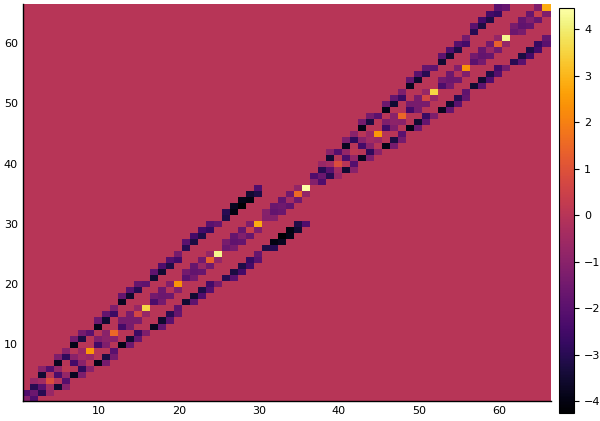
\includegraphics[width=8cm, height=7cm]{ham.png}
    \end{center}
   


    V této bázi ale $\hat{H}_D$ blokově diagonálně není, neboť

    $$\hat{H}_D^{(Nnl)} = U_D \hat{H}_D^{(\text{diagonální})} U_D^{-1} = U_D \hat{H}_R^{(\text{diagonální})} U_D^{-1} $$
    $$\hat{H}_R^{(Nnl)} = S \hat{H}_D^{(\text{blokově diagonální})} S^{-1} =  S U \hat{H}_R^{(\text{diagonální})} U^{-1} S^{-1} 
    = S U \hat{H}_D^{(\text{diagonální})} U^{-1} S^{-1}  = S U U_D^{-1} \hat{H}_D^{(Nnl)}U_D U^{-1} S^{-1} $$
Tedy 

$$\hat{H}_D^{(\text{blokově diagonální})} = U U_D^{-1} \hat{H}_D^{(Nnl)}U_D U^{-1}.$$

Vibronový hamiltonián je tak blokově diagonální v bázi $U_D U^{-1}$ (její podoba je závislá na parametrech hamiltoniánu).
   
\subsection{Blokově diagonální $\hat{H}_D$}

Bázi $\{\ket{n l} \pm \ket{n-l}\}$ označíme jako $\ket{nl\pm}$. Působení interakčních operátorů je

\begin{align*}
    \hat{R}_x \ket{nl\pm} =&
\frac{1}{\sqrt{2}}\bigg[
\sigma \bigg(\sqrt{\frac{n + j}{2} + 1} \ket{(n+1) (l+1) \pm} - \sqrt{\frac{n - j}{2} + 1} \ket{(n+1) (l-1) \pm}\bigg)  \\
 &+\sigma^{\dagger} \bigg(\sqrt{\frac{n + j}{2}} \ket{(n-1) (l-1) \pm} - \sqrt{\frac{n - j}{2}} \ket{(n-1) (l+1) \pm}\bigg)   
\bigg]
\end{align*}

\begin{align*}
    \hat{D}_x \ket{nl\pm} =&
\frac{1}{\sqrt{2}}\bigg[
\sigma \bigg(\sqrt{\frac{n + j}{2} + 1} \ket{(n+1) (l+1) \mp} - \sqrt{\frac{n - j}{2} + 1} \ket{(n+1) (l-1) \mp}\bigg)  \\
 &+\sigma^{\dagger} \bigg(\sqrt{\frac{n + j}{2}} \ket{(n-1) (l-1) \mp} - \sqrt{\frac{n - j}{2}} \ket{(n-1) (l+1) \mp}\bigg)   
\bigg]
\end{align*}

Operátor $\hat{R}_x$ tedy nemíchá kladný $\ket{nl+}$ a záporný podprostor $\ket{nl-}$, zatímco $\hat{D}_x$ ano. 

Kvantová čísla $n$ $l$, která číslují
stavy $\ket{Nnl}$, mohou být ve stavu obě sudá, nebo obě lichá. Pokud alternování sudosti a lichosti spojíme
s alternováním znaménka $\pm$ stavu  $\ket{nl\pm}$, dostaneme invariantní podprostory pro operátor 
$\hat{D}_x$.

Operátor $\hat{D}_x$ je tedy blokově diagonální ve stejné bázi, jen musíme vektory přeuspořádat.
Operátor $\hat{D}_x$ je blokově diagonální v podprostorech  
$$\text{1. podprostor} = \{\ket{nl+}_{\text{n,l - sudé}}, \ket{nl-}_{\text{n,l - liché}}\}$$
$$\text{2. podprostor} = \{\ket{nl+}_{\text{n,l - liché}}, \ket{nl-}_{\text{n,l - sudé}}\}$$

\begin{center}
    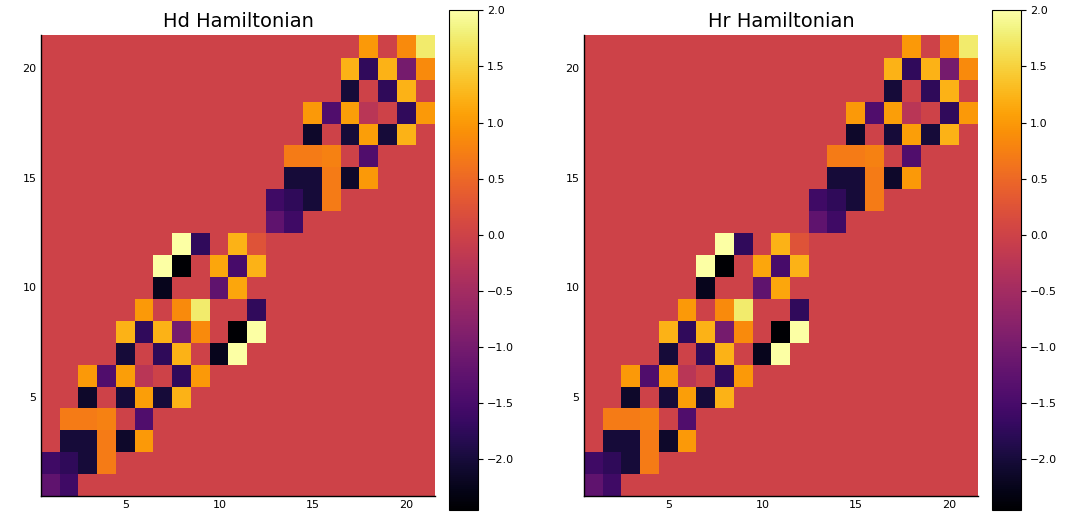
\includegraphics[width=16cm, height=7cm]{Figure_1.png}
\end{center}

Vidíme, že první podprostor je větší, protože obsahuje stavy $\ket{Nnl = 0}$ - odpovídají sudému $l$ a $\ket{l} + \ket{-l}$. Pokud
bychom je odebrali, oba bloky vypadají identicky.

\section{Závěr}
    Operátory $\hat{D}_{x,y}$ a $\hat{R}_{x,y}$ ruší degeneraci spektra a hamiltoniány $H_D$ (Iachello) a $H_R$ (Bose-Einsteinův kondenzát)
    mají stejná spektra, ale odlišné vlastní báze. 
     \end{document}
